\subsection{Background}

\begin{frame}{Background theories}
    \begin{itemize}
        \item Collaborative learning
        \item Concept mapping to support collaboration
        \item Kit-Build concept mapping approach
    \end{itemize}
\end{frame}

\begin{frame}{Why collaborative learning is important?}

    \begin{figure}[tb]
        \begin{center}
            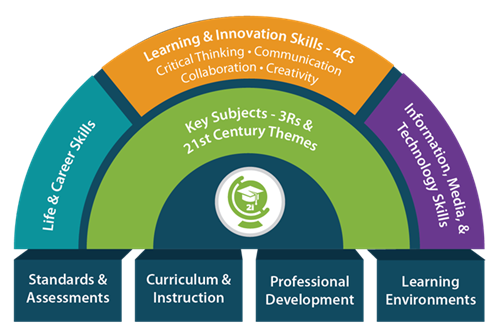
\includegraphics[width=70mm]{images/p21centuryskills.png}
        \end{center}
        \caption{Partnership for 21st century learning. Source: https://www.battelleforkids.org/networks/p21}
        \label{intro::p21}
    \end{figure}
\end{frame}

\begin{frame}{Why collaborative learning is important?}

    \begin{itemize}
        \item<1->  Collaboration is one of the \textcolor{blue}{four-essential skills} in 21st century skills
        \item<1->  The advancement of technology and rapidly changing environment require 
        collaborative works of multidisciplinary experts to solve complex problems effectively
        \item<2->  Collaboration \textcolor{blue}{does not merely happen} just because individuals are co-present
        \item<2->  It is indeed necessary to practice collaboration in the classroom
    \end{itemize}
\end{frame}

\begin{frame}{Designing learning activities to encourage collaboration}
    \begin{itemize}
        \item<1-> Students' \textcolor{blue}{interactions} play a fundamental role in collaborative learning 
        \cite{Baines2009ImprovingStudy,Webb2009TheClassroom}
        \item<1-> Various instructional strategies are employed to encourage learners to collaborate 
        (i.e. scripts, scenarios, representational tools).
        \item<2-> \textcolor{purple}{During collaboration individual learners need to make a continuous effort 
        to construct and maintain group-shared knowledge \cite{Roschelle1995TheSolving}}. 
        \item<2-> They may have forgotten prior discussion or feeling difficult to remember 
        what they have discussed or co-constructed \cite{Jeong2016SevenHelp}.
    \end{itemize}
\end{frame}

\begin{frame}{Applying concept map for collaboration}

    % add concept map figures
    \begin{figure}[tb]
        \begin{center}
            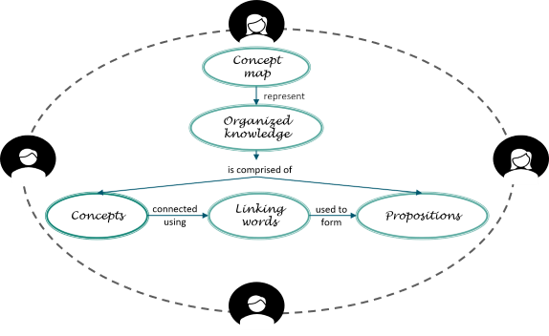
\includegraphics[width=70mm]{images/ccm.png}
        \end{center}
        \caption{An external representation tool (e.g. concept map) \textcolor{blue}{assist the learner} in articulating and \textcolor{blue}{maintaining shared focus} during discourse \cite{Fischer2002FosteringTools,Suthers2006TechnologyCSCL,vanBoxtel2002CollaborativeDiscourse}}
        \label{intro::ccm}
    \end{figure}
\end{frame}   

\begin{frame}{Collaborative concept mapping}  
    \begin{itemize}
        % \item<+-> An external representation tool \textcolor{blue}{assist the learner} in articulating and \textcolor{blue}{maintaining shared focus} during discourse \cite{Fischer2002FosteringTools,Suthers2006TechnologyCSCL,vanBoxtel2002CollaborativeDiscourse}
        % \item<+-> A concept map is a graphical tool for organizing and representing knowledge which consists of concepts and relationships among  concepts to facilitate meaningful learning \cite{novak1984learning}.
        \item<1-2> A concept map has been widely used as a representational tool to \textcolor{blue}{facilitate group discussion}, as well as to \textcolor{teal}{communicate complex ideas} \cite{Fischer2002FosteringTools,Gracia-Moreno2017CollaborativeWorkspaces,Suthers2006TechnologyCSCL,vanBoxtel2000CollaborativeKnowledge}

        \item<2> Previous studies posited that concept mapping has a positive effect on both \textcolor{teal}{students’ attitudes and learning achievements} \cite{Basque2006CollaborativeTrends,Czerniak1998TheScience}.
        
        \item<3-> However, conflicting evidence has also been found, indicating that students spend a \textcolor{purple}{considerable amount of time} focusing on task collaboration, procedure coordination, and team coordination, rather than on discussions about the concepts or relationships involved \cite{chiu2003exploring}. 
        
        \item<4> Others have also found that students encountered difficulties in \textcolor{purple}{sharing developed ideas and integrating} them into public knowledge \cite{Gracia-Moreno2017CollaborativeWorkspaces,vanBoxtel2000CollaborativeKnowledge} $\longrightarrow$ some \textcolor{purple}{inaccurate ideas are never challenged} and can become ingrained \cite{roth1992social}.
    \end{itemize}
\end{frame}

\begin{frame}{Kit-Build (KB) concept mapping approach \cite{Hirashima2015}}

    % add concept map figures
    \begin{figure}[tb]
        \begin{center}
            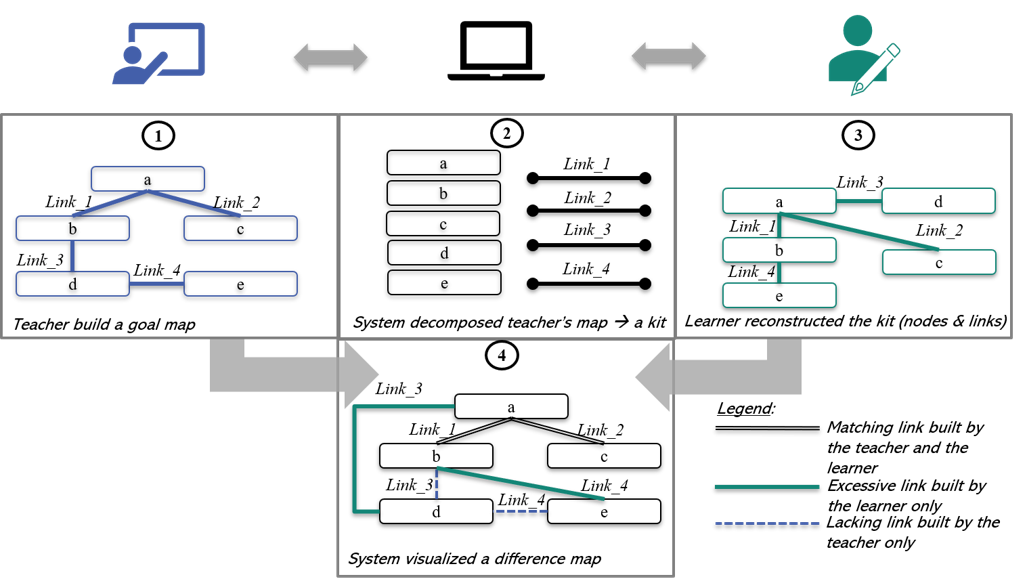
\includegraphics[width=90mm]{images/kb_flow.png}
        \end{center}
        \caption{The KB is a \textcolor{blue}{re-constructional closed-ended approach} to concept mapping
        in which students construct a map based on predefined nodes and
        links extracted from an expert's map \cite{Hirashima2015,Hirashima2019ReconstructionalReconstruction}}
        \label{intro::kbmap}
    \end{figure}
\end{frame}

\begin{frame}{Applying KB concept map for collaboration}
    \begin{itemize}
        \item<1> The KB approach enables teacher to \textcolor{blue}{confirm students' understanding}
        of the information delivered by him/her. 
        \item<2> Moreover, re-construction activity provide means to externalize 
        one's understanding on the perspective of other.
        \item<3> We believe that by applying KB map approach for peer-to-peer collaboration  $\longrightarrow$ foster \textcolor{teal}{an empathetic and effective communication}, students have \textcolor{teal}{more focus on misunderstanding}

    \end{itemize}
\end{frame}

\begin{frame}{Empathetic collaboration with KB approach}
    \begin{itemize}
        \item <+-> Effective \textcolor{blue}{collaboration} is fueled by \textcolor{teal}{empathy} 
        \item  <+-> To come up with truly  innovative solutions requires new ideas (\textcolor{blue}{creativity}). 
        \item  <+-> To bring new ideas 
        to light requires seeking a diversity of perspectives (\textcolor{blue}{critical thinking})
        and creating a welcoming space for people to share 
        their ideas without fear of judgment (\textcolor{blue}{communication}).
    \end{itemize}
\end{frame}

\begin{frame}{Reciprocal Kit Build (RKB) approach}
    An extended version of KB map approach which has been \textcolor{teal}{designed for pair discussion}
    \begin{figure}[tb]
        \begin{center}
            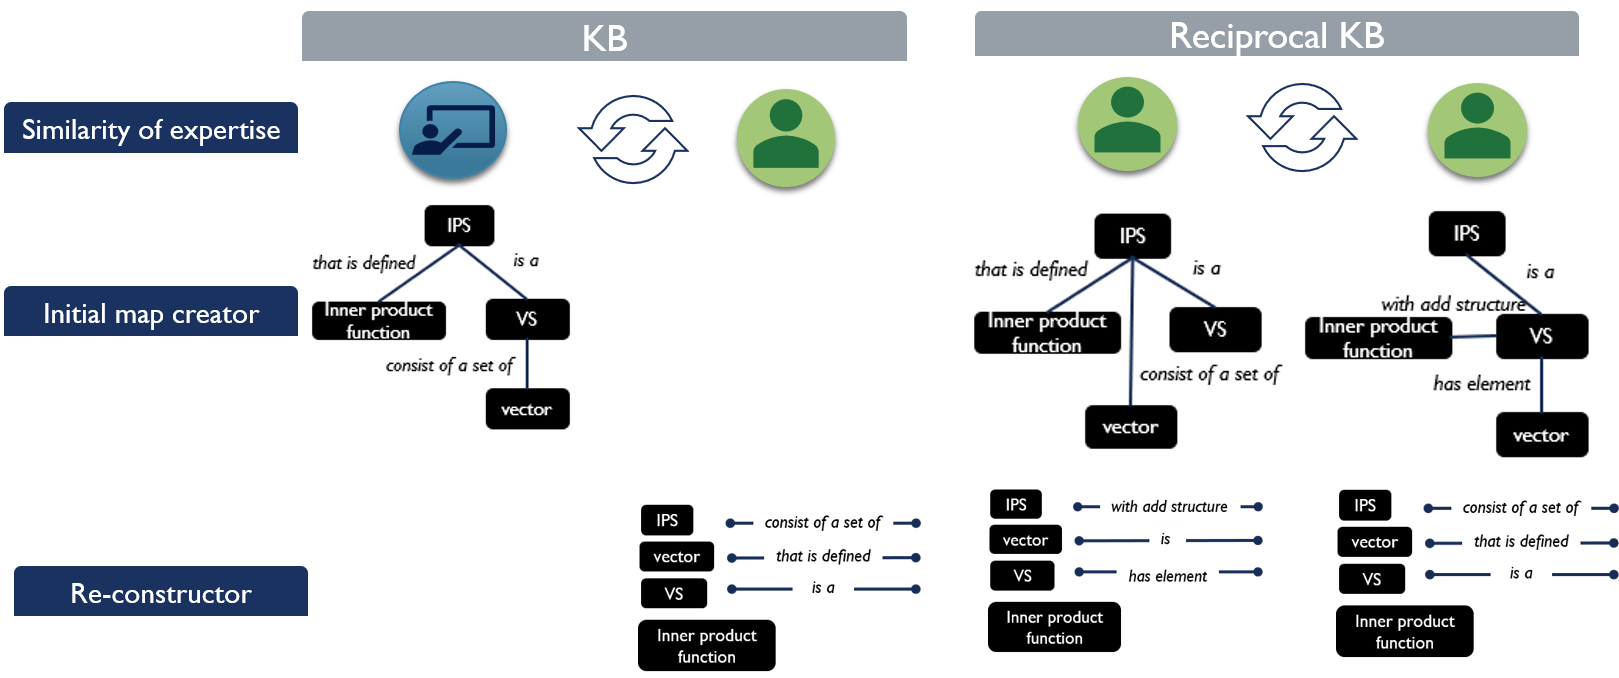
\includegraphics[width=110mm]{images/kb_rkb.pdf}
        \end{center}
        \caption{Differences between KB and RKB}
        \label{intro::kb_rkb}
    \end{figure}
    
\end{frame}


\subsection{Challenges}

\begin{frame}{Initial research on RKB}
    \begin{itemize}
        \item <1-3> Initial studies showed that the RKB approach \textcolor{blue}{promoted productive
        discussion} between partners compared to the group without reconstruction
        and difference map-supported discussion
        \cite{Wunnasri2018ReciprocalUnderstanding}. 
        \item <2-3>The RKB map also \textcolor{blue}{encouraged the pair of partners to understand each other} based on the similarity
        score of the individual's map after discussion
        \cite{Wunnasri2018ReciprocalCollaboration}. 
        \item <3-> Their findings demonstrated that the RKB can be used to \textcolor{teal}{share understanding as preparation for
        collaboration}. 
        \item <4->However, \textcolor{purple}{they have not evaluated the effect of applying
        this approach to collaborative knowledge building}, so far. 
        
    \end{itemize}
\end{frame}

\begin{frame}{Remaining problems}
    \begin{enumerate}
        \item \textcolor<1>{blue}{Collaborative products evaluation\\} 
        {\small After following RKB activities, 
        whether or not students are able to achieve high-quality group products?}
        
        \item \textcolor<2>{blue}{Students' perspective toward the activities\\} 
        {\small How is the affective response of students toward the proposed activities? An evaluation regarding students' acceptance is as important as the learning product itself. }
        \end{enumerate}
\end{frame}    
\begin{frame}{Remaining problems (cont'd)}
    \begin{enumerate}\setcounter{enumi}{2}
        \item \textcolor<1> {blue}{Investigation on the effect of different group formation effect to group collaboration\\}
        {\small To what extent, the similarity of knowledge among group members would influence collaboration? By doing so, we could determine appropriate group settings.} 
        \item \textcolor<2> {blue}{Finding factor to consider for designing support function for collaboration\\}
        {\small During the RKB session, each learner builds an individual map for two times. Which part of KB is a stronger predictor to estimate group products? How students utilize the individual maps when building a collaborative product?} 
    \end{enumerate}
\end{frame}

\subsection{Research objectives}
\begin{frame}{Research objectives}
    This study aims to identify the effect of the RKB approach
    for collaborative learning
    The purposes of this study are as follow:
    \begin{itemize}
        \item <+-> to identify the effect of the RKB approach on collaborative 
              concept mapping in a practical classroom.
        \item <+-> to investigate how individual differences in prior knowledge 
              may influence collaborative-learning effectiveness 
              (e.g. transfer of knowledge, lost knowledge, group product) 
              and the students' affective responses toward the activities. 
        \item <+-> to investigate how individual prior knowledge convergence and comprehension 
            levels through reconstruction may potentially predict the final 
            collaborative product. 
    \end{itemize} 
\end{frame}